
\section{Software Architecture}

\begin{frame}
\frametitle{Software Architecture}
The implementation of a functional architecture must consider several layers
of software architecture, where many implementation details affect the
performance of the system.\\
\vspace{0.1cm}
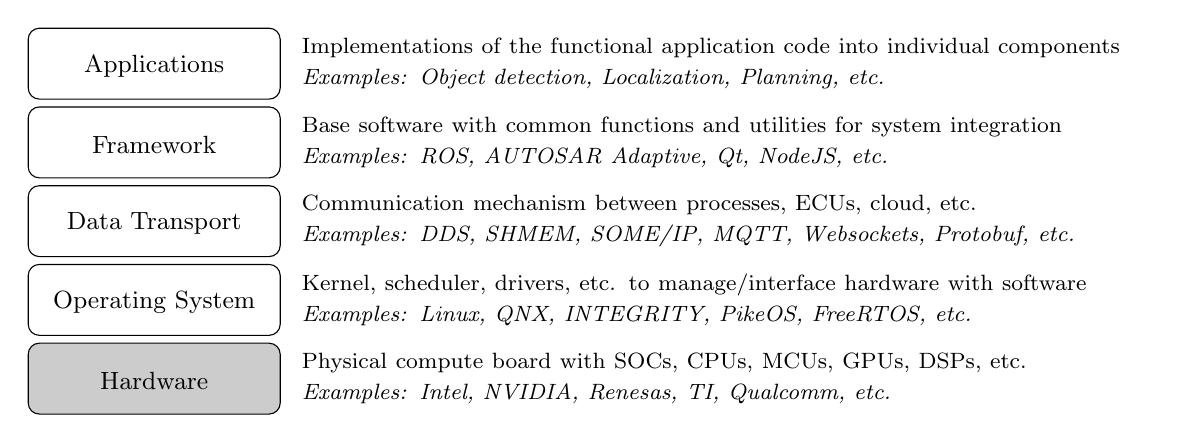
\begin{tikzpicture}[node distance=1cm,font=\small,
    layer/.style={
        draw=black,
        fill=white,
        rounded corners,
        minimum width=3.2cm,
        minimum height=0.9cm,
        text centered,
        text height=8pt},
    layerdark/.style={layer, fill=gray!40},
    ]
    \node[layer] (Apps) {Applications};
    \node[layer, below of=Apps] (FW) {Framework};
    \node[layer, below of=FW] (MW) {Data Transport};
    \node[layer, below of=MW] (OS) {Operating System};
    \node[layerdark, below of=OS] (HW) {Hardware};
    \node (AppsDesc) [right of=Apps, text width=10.75cm, xshift=6.25cm]{
        \footnotesize
        Implementations of the functional application code into individual
        components\\
        \emph{Examples: Object detection, Localization, Planning, etc.}
    };
    \node[right of=FW, text width=10.75cm, xshift=6.25cm] (FWDesc) {
        \footnotesize
        Base software with common functions and utilities for
        system integration\\
        \emph{Examples: ROS, AUTOSAR Adaptive, Qt, NodeJS, etc.}
    };
    \node[right of=MW, text width=10.75cm, xshift=6.25cm] (MWDesc) {
        \footnotesize
        Communication mechanism between processes, ECUs, cloud, etc.\\
        \emph{Examples: DDS, SHMEM, SOME/IP, MQTT, Websockets, Protobuf, etc.}
    };
    \node[right of=OS, text width=10.75cm, xshift=6.25cm] (OSDesc) {
        \footnotesize
        Kernel, scheduler, drivers, etc. to manage/interface hardware with
        software\\
        \emph{Examples: Linux, QNX, INTEGRITY, PikeOS, FreeRTOS, etc.}
    };
    \node[right of=HW, text width=10.75cm, xshift=6.25cm] (HWDesc) {
        \footnotesize
        Physical compute board with SOCs, CPUs, MCUs, GPUs, DSPs, etc.\\
        \emph{Examples: Intel, NVIDIA, Renesas, TI, Qualcomm, etc.}
    };
\end{tikzpicture}
\end{frame}

\begin{frame}
\frametitle{Software Frameworks for Autonomous Driving}
\framesubtitle{Framework requirements}
What are some of the functions, utilities and APIs that an application requires?
\vspace{0.25cm}
\begin{itemize}
    \item Concept of partitioning a larger system into components
    \item Means of receiving and transmitting data between components
    \item Configuration / parametrization of components
    \item Management of component execution und underlying CPU resources,
        e.g. threads
    \item Tools for development, debugging, and deployment
    \item Compatible with different programming languages and platforms
\end{itemize}
\end{frame}

\begin{frame}
\frametitle{Software Frameworks for Autonomous Driving}
\framesubtitle{Today's most popular solutions}
\centering
\begin{columns}[]
    \begin{column}{0.33\textwidth}
        \centering
        
\includegraphics[width=0.8\textwidth]{images/logo_ros.png}\\
    \end{column}
    \begin{column}{0.33\textwidth}
        \centering
        
\includegraphics[width=0.9\textwidth]{images/logo_mathworks.jpg}\\
    \end{column}
    \begin{column}{0.33\textwidth}
        \centering
        
\includegraphics[width=0.3\textwidth]{images/logo_elektrobit.jpg}\\
    \end{column}
\end{columns}
\vspace{0.2cm}
\begin{columns}[]
    \begin{column}{0.33\textwidth}
        \centering
        \footnotesize
        Robot Operating System\footnotemark[1]\\
    \end{column}
    \begin{column}{0.33\textwidth}
        \centering
        \footnotesize
        MATLAB/Simulink\footnotemark[2]
    \end{column}
    \begin{column}{0.33\textwidth}
        \centering
        \footnotesize
        EB Assist ADTF\footnotemark[3]
    \end{column}
\end{columns}
\vspace{0.25cm}
\begin{columns}[]
    \begin{column}{0.33\textwidth}
        \centering
        
\includegraphics[width=0.9\textwidth]{images/logo_autosar.png}\\
    \end{column}
    \begin{column}{0.33\textwidth}
        \centering
        
\includegraphics[width=0.6\textwidth]{images/logo_nvidia.png}\\
    \end{column}
    \begin{column}{0.33\textwidth}
        \centering
        
\includegraphics[width=0.8\textwidth]{images/logo_motionwise.png}\\
    \end{column}
\end{columns}
\vspace{0.2cm}
\begin{columns}[]
    \begin{column}{0.33\textwidth}
        \centering
        \footnotesize
        AUTOSAR\footnotemark[4]
    \end{column}
    \begin{column}{0.33\textwidth}
        \centering
        \footnotesize
        NVIDIA DriveWorks\footnotemark[5]
    \end{column}
    \begin{column}{0.33\textwidth}
        \centering
        \footnotesize
        TTTech Auto MotionWise\footnotemark[6]
    \end{column}
\end{columns}
\footnotetext[1]{\tiny{\url{https://ros.org/}}}
\footnotetext[2]{\tiny{\url{https://www.mathworks.com/products/automated-driving.html}}}
\footnotetext[3]{\tiny{\url{https://www.elektrobit.com/products/automated-driving/eb-assist/adtf/}}}
\footnotetext[4]{\tiny{\url{https://www.autosar.org/}}}
\footnotetext[5]{\tiny{\url{https://developer.nvidia.com/drive/driveworks}}}
\footnotetext[6]{\tiny{\url{https://www.tttech-auto.com/products/safety-software-platform/motionwise/}}}
\end{frame}

\begin{frame}
\frametitle{Software Frameworks for Autonomous Driving}
\framesubtitle{Today's most popular solutions}
\begin{center}
    
\includegraphics[width=0.4\textwidth]{images/logo_apexai.png}
\end{center}
\vspace{0.25cm}
Apex.AI\footnotemark[1] has developed Apex.OS\footnotemark[2] and
Apex.Middleware\footnotemark[3], a software framework and
middleware based on ROS and designed for safety-certified automotive
applications.
\footnotetext[1]{\tiny{\url{https://www.apex.ai/}}}
\footnotetext[2]{\tiny{\url{https://www.apex.ai/apex-os}}}
\footnotetext[3]{\tiny{\url{https://www.apex.ai/apex-middleware}}}
\end{frame}

\subsection{ROS}

\begin{frame}
\frametitle{Robot Operating System (ROS)}
\framesubtitle{Overview}
\begin{columns}[]
    \begin{column}{0.7\textwidth}
        \begin{itemize}
            \item Most popular framework for developing robotics (and other)
                applications
            \item Open source with thousands of contributors world wide
            \item Widely adopted by universities, research institutes and
                and companies
            \item Thousands of packages\footnotemark[1] (applications) for
                sensors, perception, SLAM, motion planning, etc.
            \item Powerful suite of tools (visualization, introspection,
                debugging, etc.)
            \item Wide support for different programming languages
            \item Hundreds of autonomous vehicles in R\&D run on ROS
        \end{itemize}
    \end{column}
    \begin{column}{0.3\textwidth}
        \centering
        
\includegraphics[width=\textwidth]{images/logo_ros.png}
    \end{column}
\end{columns}
\footnotetext[1]{\tiny{\url{https://index.ros.org/packages/}}}
\end{frame}

\begin{frame}
\frametitle{Robot Operating System (ROS)}
\framesubtitle{The basics}
\begin{columns}[]
    \begin{column}{0.5\textwidth}
        \begin{itemize}
            \item \textbf{Nodes}: A single processing entity with inputs and
                outputs
            \item \textbf{Topics}: Data channels between nodes
            \item \textbf{Messages}: The data type which is transmitted on a
                topic
            \item \textbf{Publisher}: Within a node, the entity that transmits
                data on a topic
            \item \textbf{Subscriber}: Within a node, the entity that receives
                data on a topic
            \item \textbf{Service}: Request/response mechanism between nodes
        \end{itemize}
    \end{column}
    \begin{column}{0.5\textwidth}
        \centering
        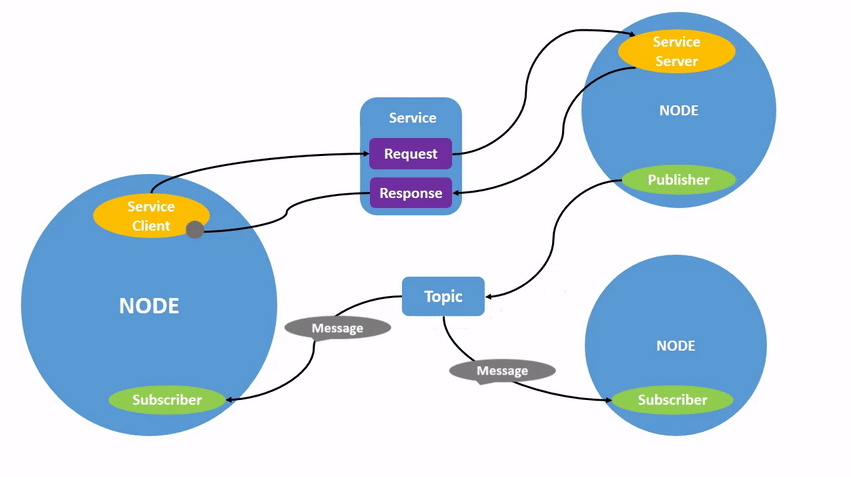
\includegraphics[width=\textwidth]{images/ros_overview.png}
        \tiny{Source: ROS 2 Tutorials - Understanding ROS 2 nodes\footnotemark[1]}
    \end{column}
\end{columns}
\footnotetext[1]{\tiny{\url{https://docs.ros.org/en/galactic/Tutorials/Understanding-ROS2-Nodes.html}}}
\end{frame}

\begin{frame}[fragile]
\frametitle{Robot Operating System (ROS)}
\framesubtitle{Example ROS 2 node in C++}
\tiny
\begin{minted}{cpp}
// From https://docs.ros.org/en/galactic/Tutorials/Writing-A-Simple-Cpp-Publisher-And-Subscriber.html
class MinimalPublisher : public rclcpp::Node {
    public:
        MinimalPublisher() : Node("minimal_publisher"), count_(0) {
            publisher_ = this->create_publisher<std_msgs::msg::String>("topic", 10);
            timer_ = this->create_wall_timer(500ms, std::bind(&MinimalPublisher::timer_callback, this));
        }
    private:
        void timer_callback() {
            auto message = std_msgs::msg::String();
            message.data = "Hello, world! " + std::to_string(count_++);
            RCLCPP_INFO(this->get_logger(), "Publishing: '%s'", message.data.c_str());
            publisher_->publish(message);
        }
        rclcpp::TimerBase::SharedPtr timer_;
        rclcpp::Publisher<std_msgs::msg::String>::SharedPtr publisher_;
        size_t count_;
};

int main(int argc, char * argv[]) {
    rclcpp::init(argc, argv);
    rclcpp::spin(std::make_shared<MinimalPublisher>());
    rclcpp::shutdown();
    return 0;
}
\end{minted}
\end{frame}

\begin{frame}
\frametitle{Robot Operating System (ROS)}
\framesubtitle{Tools}
\begin{columns}[]
    \begin{column}{0.65\textwidth}
        \footnotesize
        ROS has a rich suite of tools, both included in the standard installation as
        well as tools developed by the community.\\
        \begin{itemize}
            \item Command line tools for system introspection, configuration,
                and launching
            \item rosbag\footnotemark[1] recording and replay tool
            \item RViz\footnotemark[2]: 3D Visualizer
            \item rqt\footnotemark[3]: Qt based GUI with customizable plug-ins
            \item Robot Web Tools\footnotemark[4]: web based interfacing with ROS
            \item PlotJuggler\footnotemark[5]: plotting of ROS message data 
        \end{itemize}
    \end{column}
    \begin{column}{0.35\textwidth}
        \centering
        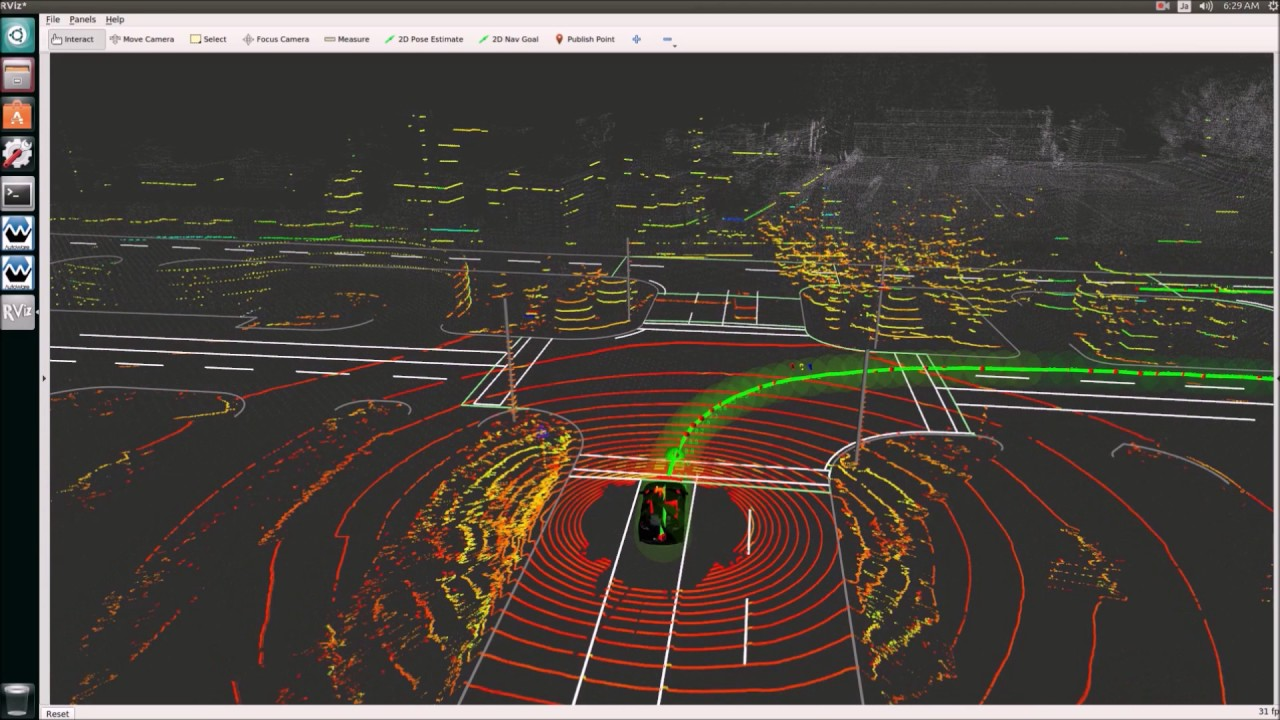
\includegraphics[width=0.6\textwidth]{images/rviz.jpg}\\
        \scriptsize RViz\footnotemark[2] 3D Visualizer\\
        Source: YouTube (Autoware)\footnotemark[6]\\
        \vspace{0.25cm}
        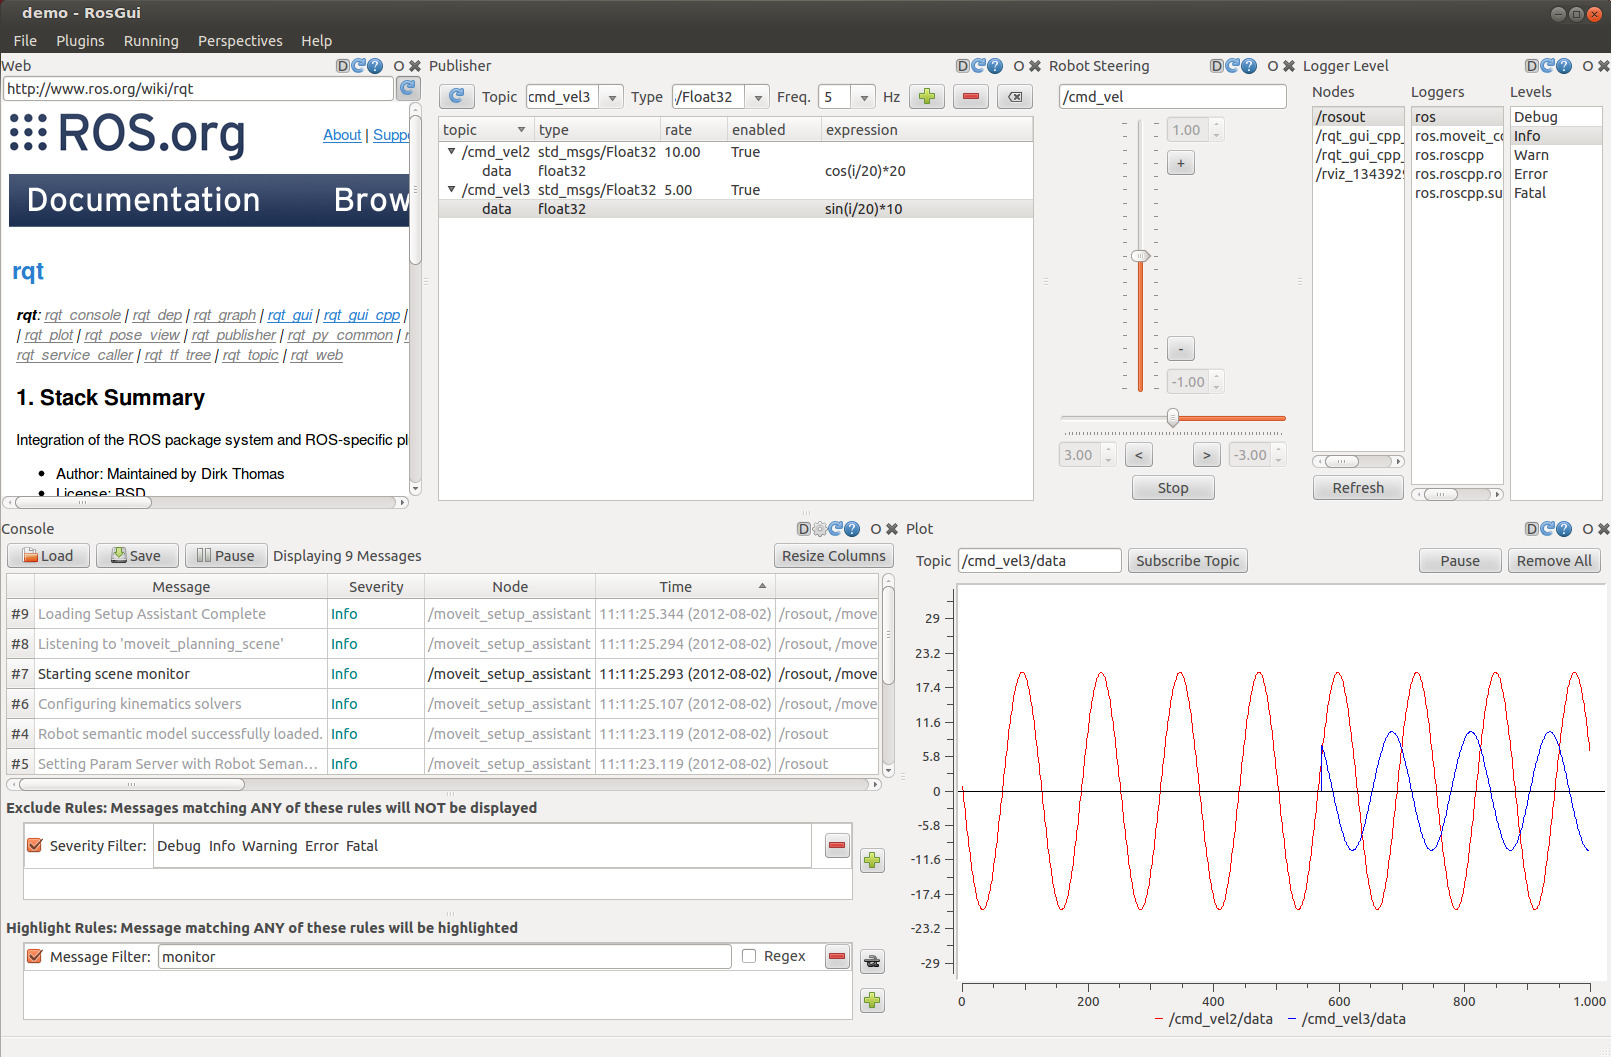
\includegraphics[width=0.6\textwidth]{images/rqt.png}\\
        \scriptsize rqt\footnotemark[3] GUI
    \end{column}
\end{columns}
\footnotetext[1]{\tiny{\url{https://github.com/ros2/rosbag2}}}
\footnotetext[2]{\tiny{\url{https://github.com/ros2/rviz}}}
\footnotetext[3]{\tiny{\url{http://wiki.ros.org/rqt}}}
\footnotetext[4]{\tiny{\url{http://robotwebtools.org/}}}
\footnotetext[5]{\tiny{\url{https://www.plotjuggler.io/}}}
\footnotetext[6]{\tiny{\url{https://www.youtube.com/watch?v=zujGfJcZCpQ}}}
\end{frame}

\subsection{Production Frameworks}

\begin{frame}
\frametitle{Production Software Frameworks}
A software framework and middleware for a production vehicle has many
additional requirements that need to be met.

\begin{itemize}
    \item Safety requirements and standards must be met
    \item Software must run on embedded hardware with limited resources
    \item Automotive interfaces must be supported (CAN, LIN, automotive
        Ethernet, etc.)
    \item Security requirements must be met, e.g. end-to-end protection, 
        identity access management, etc.
    \item Automotive interfaces such as Unified Diagnostics Service (UDS) must
        be implemented
\end{itemize}
\end{frame}

\begin{frame}
\frametitle{AUTOSAR Classic}
AUTOSAR was formed in 2003 to standardize automotive E/E architecture.
Applications can be developed against a standard Runtime Environment
for automotive \emph{microcontrollers}.
\begin{center}
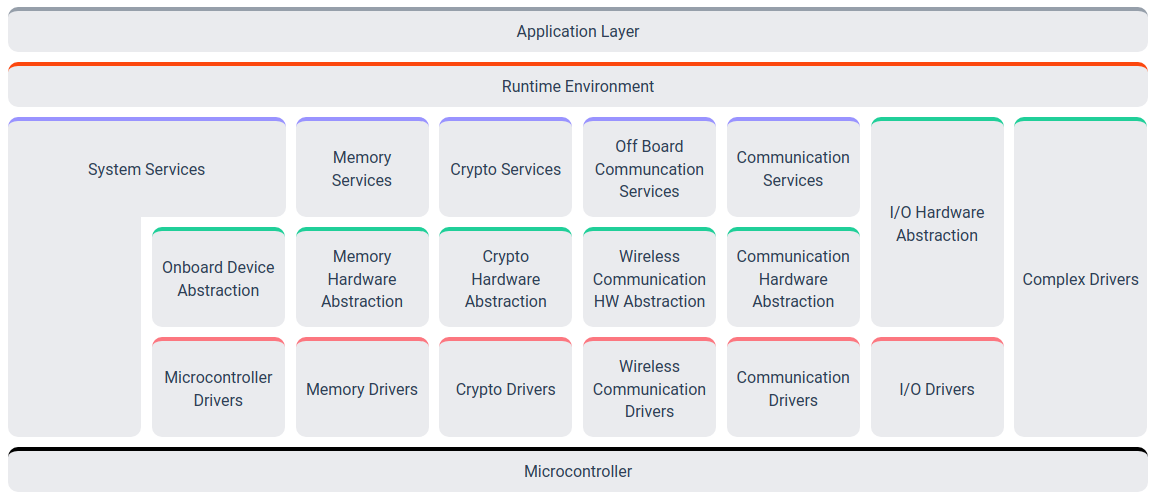
\includegraphics[width=0.75\textwidth]{images/autosar_classic.png}\\
\footnotesize  Source: AUTOSAR Classic Platform\footnotemark[1]
\end{center}
\footnotetext[1]{\tiny{\url{https://www.autosar.org/standards/classic-platform/}}}
\end{frame}

\begin{frame}
\frametitle{AUTOSAR Adaptive}
Next-generation of AUTOSAR designed for high performance computing hardware
running with a POSIX based operating system. Uses a service oriented
architecture.
\begin{center}
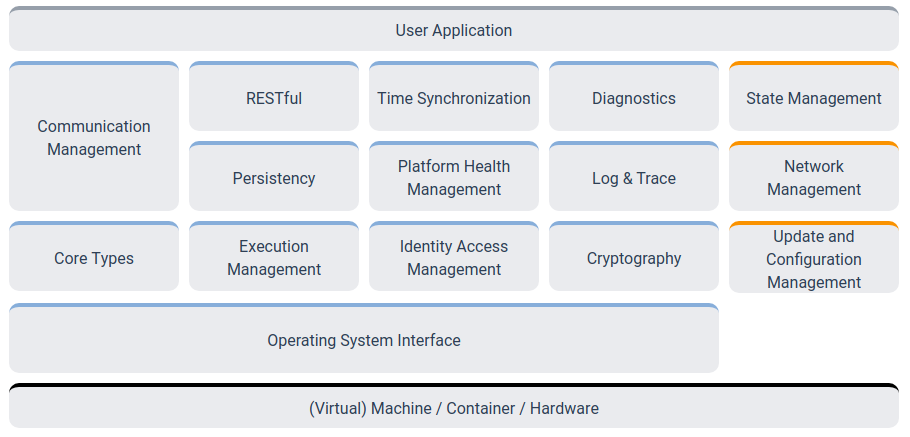
\includegraphics[width=0.7\textwidth]{images/autosar_adaptive.png}\\
\footnotesize Source: AUTOSAR Classic Platform\footnotemark[1]
\end{center}
\footnotetext[1]{\tiny{\url{https://www.autosar.org/standards/adaptive-platform/}}}
\end{frame}

\begin{frame}
\frametitle{Apex.OS}
Apex.OS is a production framework and SDK based on ROS 2.
\begin{center}
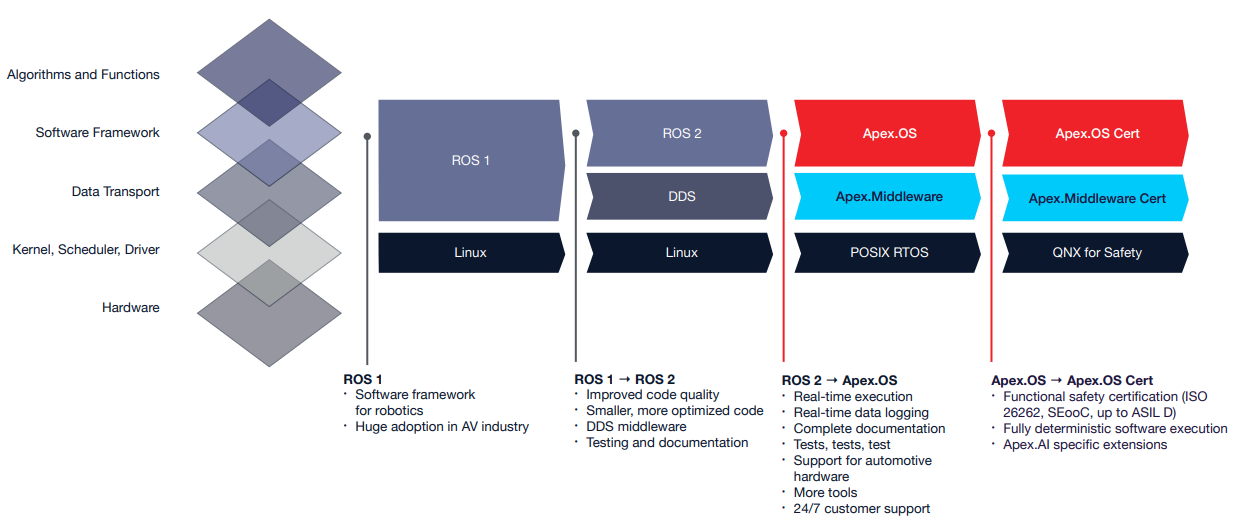
\includegraphics[width=\textwidth]{images/apex_ros_to_apexos.png}\\
\scriptsize Source: Apex.AI
\end{center}
\end{frame}

\subsection{Middleware}

\begin{frame}
\frametitle{Data Transport Middlewares}
\framesubtitle{Overview}
A complete vehicle system requires many different mechanism for transporting
data from one component to another.\\
\begin{columns}[]
    \begin{column}{0.6\textwidth}
        Middleware requirements:
        \begin{itemize}
            \item Handle GByte/s data transfer (e.g. camera images)
            \item Short latencies and low run-time resource consumption
            \item Many-to-many communication
            \item Interfacing with diverse set of protocols
        \end{itemize}
    \end{column}
    \begin{column}{0.4\textwidth}
        \centering
        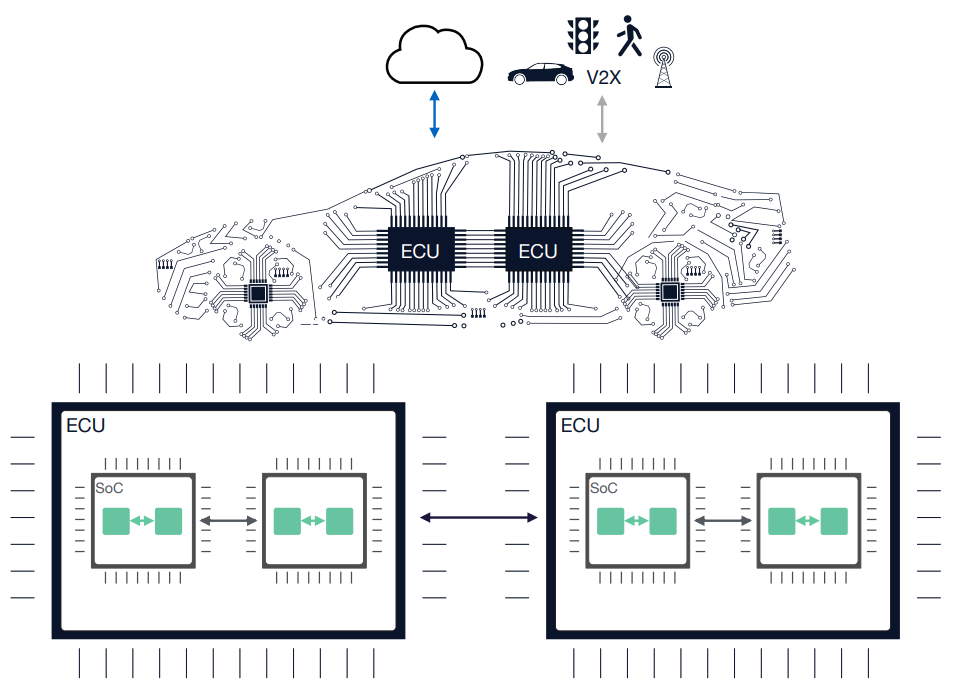
\includegraphics[width=\textwidth]{images/apex_vehicle_coms.png}\\
        \scriptsize Source: Apex.AI
    \end{column}
\end{columns}
\end{frame}

\begin{frame}
\frametitle{Data Transport Middlewares}
\framesubtitle{Automotive communication buses}
Automotive communication mechanisms are designed to be robust and reliable
where several ECUs can exchange data.
\begin{itemize}
    \item CAN: Reliable bus system to exchange small bits of data across many ECUs
    \item FlexRay: Improved performance for safety-critical systems
    \item LIN: Integration of simple sensors and actuators
    \item MOST: Designed for the transmission of multimedia data,
        e.g. video, audio, etc.
\end{itemize}
For each of these technologies, a middleware software stack is required to make
the data on the bus system available to an application. In the automotive
industry, this is often accomplished with the AUTOSAR Classic stack.
\end{frame}

\begin{frame}
\frametitle{Data Transport Middlewares}
\framesubtitle{Ethernet}
In recent years, automotive Ethernet has made it into production vehicles,
enabling the high-bandwidth data rates of Ethernet with the well-known
TCP and UDP networking protocols. Two popular software middlewares are built
on Ethernet.
\begin{columns}[T]
    \begin{column}{0.5\textwidth}
        
\includegraphics[width=0.125\textwidth]{images/dds.jpg}
        \begin{itemize}
            \item DDS\footnotemark[1] is an OMG standard
            \item Publisher/subscriber on topics
            \item Standardized interface, OMG IDL\footnotemark[2]
            \item Rich set quality of service settings
            \item Used in many industries: automotive, robotics, banking,
                medical, aerospace
        \end{itemize}
    \end{column}
    \begin{column}{0.5\textwidth}
        SOME/IP\footnotemark[3]\\
        \begin{itemize}
            \item Standardized within the scope of AUTOSAR \cite{AutosarSomeIp}
            \item Service oriented architecture
            \item Interface definition with ARXML (from AUTOSAR)
            \item No quality of service
            \item Mainly used in automotive
        \end{itemize}
    \end{column}
\end{columns}
\footnotetext[1]{\tiny{\url{https://www.dds-foundation.org/}}}
\footnotetext[2]{\tiny{\url{https://www.omg.org/spec/IDL/4.2/About-IDL/}}}
\footnotetext[3]{\tiny{\url{https://some-ip.com/}}}
\end{frame}

\begin{frame}
\frametitle{Data Transport Middlewares}
\framesubtitle{Shared memory}
For data transmission of high-bandwidth data (e.g. camera data) on the same
ECU, the copying, serialization, and deserialization of the data consumes
significant CPU resources.\\

An efficient shared memory data transport is required to reduce the CPU
overhead. The Eclipse iceoryx\texttrademark\footnotemark[1] shared memory
middleware enables constant-time true zero-copy data transport.

\begin{center}
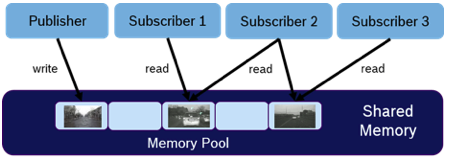
\includegraphics[width=0.5\textwidth]{images/shared_memory.png}\\
\footnotesize Source: Eclipse Foundation\footnotemark[1]
\end{center}
\footnotetext[1]{\tiny{\url{https://www.eclipse.org/community/eclipse_newsletter/2019/december/4.php}}}
\end{frame}

\begin{frame}
\frametitle{Data Transport Middlewares}
\framesubtitle{Apex.Middleware}
\begin{columns}[]
    \begin{column}{0.6\textwidth}
        A single middleware designed to communicate using different protocols
        in the context of automotive and robotics applications.
        \begin{itemize}
            \item Shared memory backbone with Eclipse iceoryx\texttrademark\footnotemark[1]
            \item Ethernet communication with Eclipse Cyclone DDS\texttrademark\footnotemark[2]
                and automotive SOME/IP
            \item Support for PDU communication, e.g. CAN
            \item MQTT for cloud connectivity
        \end{itemize}
    \end{column}
    \begin{column}{0.4\textwidth}
        \centering
        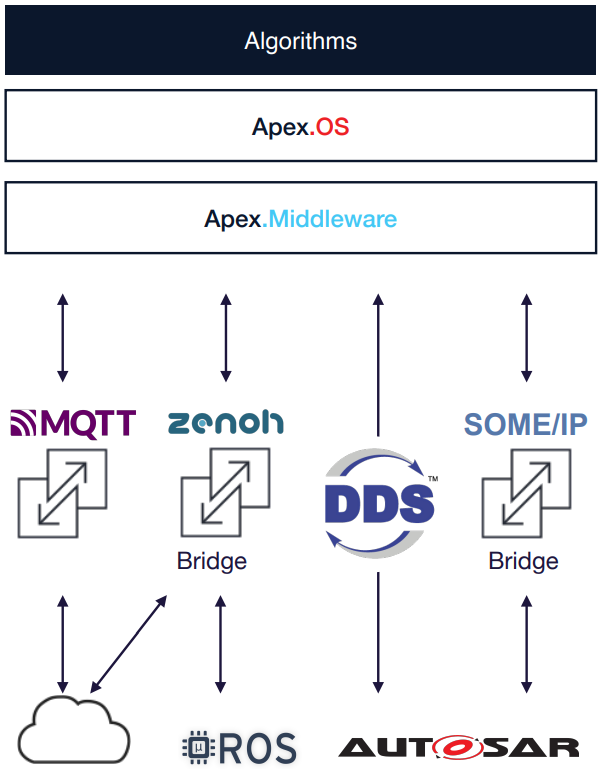
\includegraphics[width=0.8\textwidth]{images/apex_middleware.png}\\
        \scriptsize Source: Apex.AI
    \end{column}
\end{columns}
\footnotetext[1]{\tiny{\url{https://iceoryx.io/}}}
\footnotetext[2]{\tiny{\url{https://cyclonedds.io/}}}
\end{frame}

\subsection{Operating Systems}

\begin{frame}
\frametitle{Operating Systems}
The operating system is responsible for managing the interface between software
applications and the underlying hardware: memory management, process/task
management, input/output communications, etc.
\begin{columns}[]
    \begin{column}{0.7\textwidth}
        \begin{itemize}
            \item Modern high-performance computers run a
                POSIX compliant (real-time) operating system (Linux, QNX$^{\tiny{\textregistered}}$,
                INTEGRITY, PikeOS, etc.)
            \item AUTOSAR Classic OSEK \cite{ISO17356} dominates the automotive microcontrollers
            \item A Hypervisor can be used to manage several guest operating systems
                sharing the resources of a single CPU
                \begin{itemize}
                    \item Partitioning of safety and non-safety applications
                \end{itemize}
            \item Development is typically on Linux or Windows
        \end{itemize}
    \end{column}
    \begin{column}{0.3\textwidth}
        \centering
        
\includegraphics[height=2cm]{images/linux-logo.png}\\
        \scriptsize Source: Wikipedia\footnotemark[1]\\
        \vspace{0.5cm}
        
\includegraphics[width=0.9\textwidth]{images/qnx-logo.png}\\
        \scriptsize Source: Blackberry QNX$^{\tiny{\textregistered}}$\footnotemark[2]
    \end{column}
\end{columns}
\footnotetext[1]{\tiny{\url{https://en.wikipedia.org/wiki/Linux}}}
\footnotetext[2]{\tiny{\url{https://blackberry.qnx.com/en/products/safety-certified/qnx-os-for-safety}}}
\end{frame}